\chapter{The PerLa System}

\section{A brief history of PerLa}

PerLa is a software infrastructure for data management and integration in
Pervasive Information Systems. Its development began in 2005 at Politecnico di
Milano, with a thesis by Marco Marelli and Marco Fortunato entitled ``\textit{A
Declarative Language for Pervasive Systems}'' \cite{mm_thesis}. With this
document the two authors laid the foundations for a completely declarative,
SQL-like language that could be used to gather information from Pervasive
Systems and Wireless Sensing Networks alike. Though their work primarily
focussed on defining the syntax and semantics of the PerLa language, Marelli
and Fortunato went on to propose a reference software architecture that could
support the execution of PerLa data collection queries.

In their first design they envisioned the possibility of creating a
\textit{Device Access Layer}, whose goal was to conceal all the idiosyncratic
features of a Pervasive System, and provide a homogeneous data access interface
that could be used as a thought device to support the first development stages
of PerLa. The principal element of this initial software architecture was the
\textit{Logical Object}, a virtualization module that provides a uniform API
for accessing the functionalities of a single device in the sensing network;
this germinal design evolved during the course of the following years
into what would later be known as \textit{PerLa Middleware}. 

The PerLa Middleware~\cite{tse_perla} was primarily concerned with providing an
actual implementation to the Logical Object abstraction, a goal that was
achieved with the creation of the Functionality Proxy Component (\texttt{FPC}).
The \texttt{FPC} is a Java entity that reifies all concepts embodied by the
Logical Object, with particular emphasis on the ability to abstract the
peculiar features of a single sensing device through a common and uniform
programming interface. The PerLa Middleware, however, was more than a simple
implementation of the Logical Object, as it provided a \textit{Plug \& Play}
system for the autonomous creation of \texttt{FPC} objects, as well as an
initial release of the PerLa Query Executor component.

The development of the PerLa Middleware has been a collaborative effort that
involved multiple students and several years of work. Therefore, the product
that ensued is the sum of all contributions made by different people, that, at
one time or another, put their minds and hearts at the design and
implementation of the system. While such development approach allowed PerLa to
thrive and mature rapidly, since many intellects had the possibility to
contribute with their innovative ideas, it also meant that the growth of the
system has been inconstant and, at times, chaotic. It is under these premises
that, in early 2014, the Middleware underwent a complete redesign, whose
primary intentions were to consolidate the main programmatic API (Application
Programming Interface), improve performances, and further advance some of the
defining characteristics of its architecture. The document you are reading is
an account of this recent endeavor, and contains a description of the past,
present and foreseeable future of the PerLa System.

The remaining sections of this chapter provide an account of PerLa prior to the
current redesign, starting with the previous Middleware architecture --- also
known as Classic PerLa Middleware --- and ending with a short digression
towards Context management in Pervasive Systems. This same chapter will
describe the main features of the PerLa Query Language, which as of today still
is the interface of choice for using PerLa.
Chapters~\ref{cha:middleware_overview} and~\ref{cha:components} contain an
in-depth description of the New Middleware architecture, which should be of
concern to any programmer interested in developing new PerLa Plugins or
connecting new types of sensing devices. Finally, chapter~\ref{cha:conclusions}
wraps up the work illustrated in this thesis, and provides an outlook on the
prospects for PerLa's future.


\section{The Classic Middleware Architecture}

\subsection{Main goals and operating principles}

The PerLa Middleware is a complex software based on the Java platform. Its
development focussed primarily on the design and implementation of the
following features:

\begin{itemize}

    \item data-centric view of Pervasive Systems;

    \item homogeneous high level interface to heterogeneous
        devices;

    \item support for highly dynamic networks (e.g., wireless
        sensor networks);

    \item minimal coding effort for new device addition.

\end{itemize}

The remaining of this chapter will show how the implementation of the
\texttt{FPC} component and the development of a Plug \& Play device addition
mechanism contributed to achieving the aforementioned goals. The reader is
stronly encouraged not to skip these following sections, as most of the
concepts hereby introduced will be subject of further discussion in
chapter~\ref{cha:middleware_overview}, where they are going to be matched
alongside their novel counterparts.

\subsection{The Functionality Proxy Component}

As previously stated, the principal element of the PerLa Middleware, both in
its classic and redesigned incarnations, is the \texttt{FPC}. Its primary
function consists in providing a consistent and homogeneous interface that can
be used by high-level components of the PerLa System to access all
functionalities of a Pervasive System, without requiring any knowledge of the
underlying hardware layer.

All data elements accessible through an \texttt{FPC} are abstracted using the
concept of \textit{Device Attribute}, namely a single piece of information
produced or consumed by a node in the Pervasive System. By design, device
attributes are not tied to a particular technology, and can therefore be used
to represent any primitive value, regardless of the method employed for its
generation (physical sampling, read from main memory, etc.). Device Attributes
are one of the defining aspects of the PerLa Middleware, and greatly contribute
to the creation of a data-centric abstraction that can be used to access all
features of a sensing network, as any operation performed through the
\texttt{FPC} interface is specified in terms of reading or writing a specific
set of attributes.

\begin{figure}[h!]
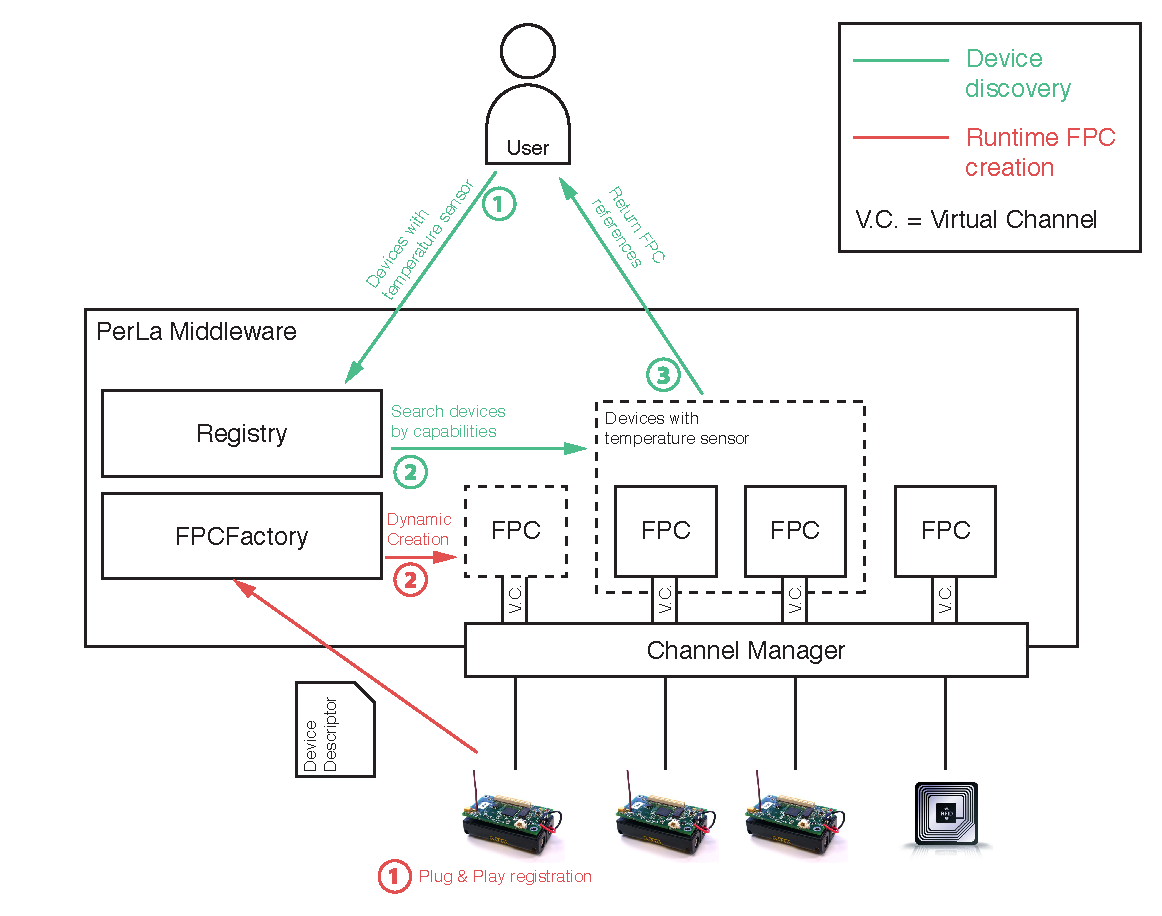
\includegraphics[width=\textwidth]{imgs/classic_middleware_overview.pdf}
\caption{The Classic PerLa Middleware architecture}
\label{fig:classic_architecture}
\end{figure}

In the Classic PerLa Middleware, the physical connection between an
\texttt{FPC} and its remote device is entirely managed by the \texttt{Channel
Manager} (see figure~\ref{fig:classic_architecture}). This singleton component
is responsible for the creation of \texttt{Virtual Channels}, abstract network
interfaces that conceal the specific technologies required to hold a
communication link between two endpoints of a Pervasive System. By means of the
\texttt{Channel Manager}, \texttt{FPC}s and physical devices can exchange
information transparently, mutually ignoring all the architectural differences
that may exist between them. The achievement of a truly universal communication
system, however, is severily limited by the capabilities of the \texttt{Channel
Manager} itself, as the choice of protocols available in the Classic Middleware
is restricted to those that the original PerLa Developers hard-coded into this
component.

\begin{figure}[h!]
\center
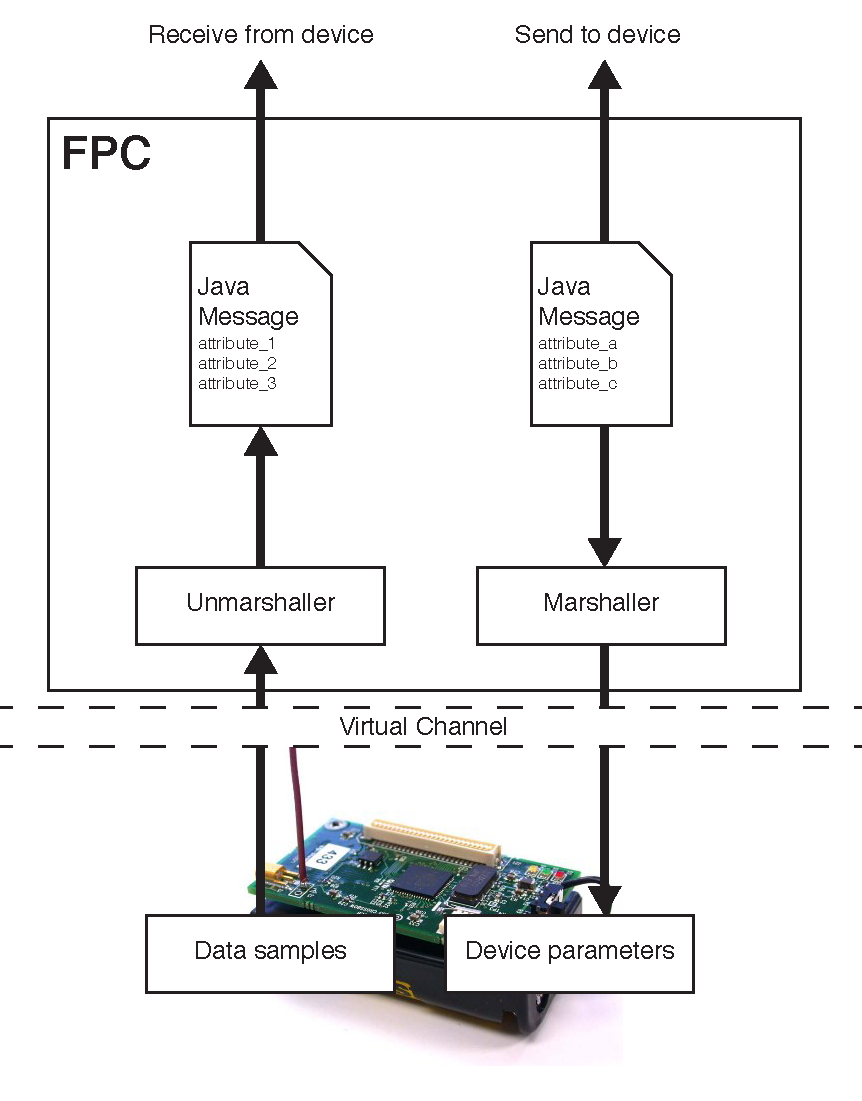
\includegraphics[width=0.6\textwidth]{imgs/classic_fpc.pdf}
\caption{The Classic FPC design}
\label{fig:classic_fpc}
\end{figure}

As shown in figure~\ref{fig:classic_fpc}, the internal structure of the Classic
\texttt{FPC} is mainly composed of a \texttt{Marshaller}, an
\texttt{Unmarshaller}, and a selection of Java objects representing the
messages which can be exchanged with the remote endpoint. This early design is
enough to implements a simplified data collection mechanism, based on the
assumptions that every device attribute can be mapped to exactly one message
field. Under the Classic Middleware, a typical data collection request for a
well-defined set of attributes would then be executed as follows:

\begin{enumerate}

    \item Starting from a user's request, and leveraging the one-to-one
        relationship between attributes and message fields, the \texttt{FPC}
        compiles a list of data structures which are to be collected from the
        remote device;

    \item The remote device starts streaming data to the \texttt{FPC}. This
        information is unmarshalled into a high-level Java message, according
        to the directives specified inside the Device Descriptor (see
        section~\ref{sec:classic_fpcfactory};

    \item All message fields containing relevant information for the user are
        read in order to produce an output record.

\end{enumerate}

A similar process, making use of the \texttt{Marshaller} component instead of
the \texttt{Unmarshaller}, and with a reversed data flow, allows the
\texttt{FPC} component to send configuration parameters towards its controlled
device.

\subsection{Plug \& Play device addition}
\label{sec:classic_fpcfactory}

Sensing nodes can be added to a running instance of the PerLa Middleware
through a \textit{Plug \& Play} device registration mechanism, that allows the
discovery and configuration of new devices without the need for direct user
interventions. This operation is performed at runtime by the
\texttt{FPCFactory}, a software component tasked with creating new \texttt{FPC}
objects from a blueprint document called \textit{Device Descriptor}.
PerLa-enabled devices are programmed to send their XML descriptor at startup;
this allows them to be readily available for use, as their controlling
\texttt{FPC} object is dynamically instantiated by the \texttt{FPCFactory} upon
reception of the Device Descriptor. Figure~\ref{fig:classic_middleware}
contains a graphic portrayal of this entire process.

\begin{figure}[h!]
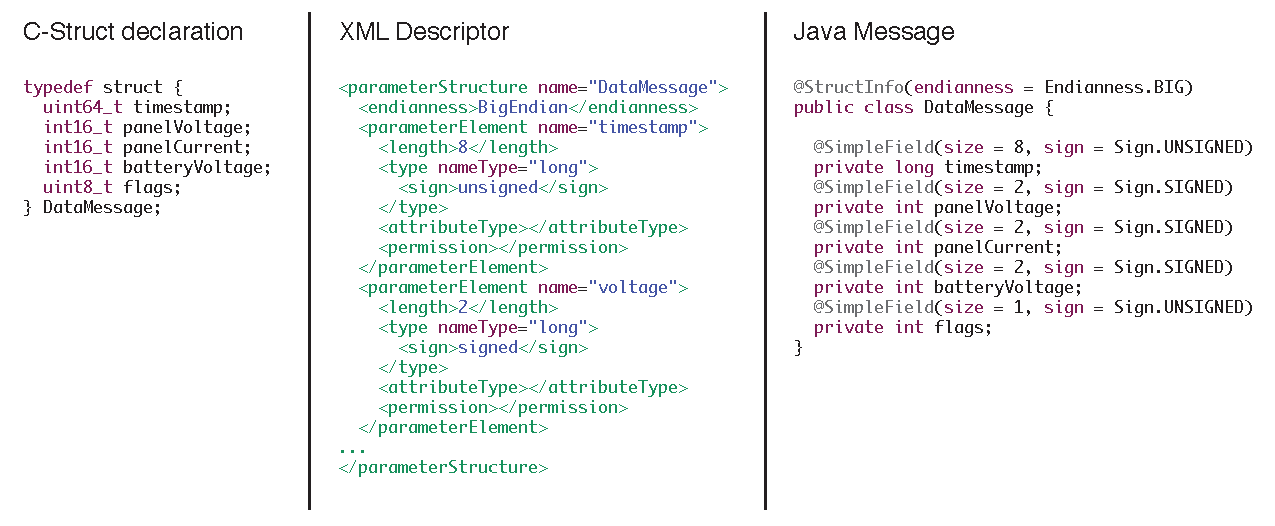
\includegraphics[width=\textwidth]{imgs/classic_descriptor.pdf}
\caption{Physical to logical attribute mapping in the Classic PerLa Middleware.
The annotations added to the Java Message allow the \texttt{Marshaller} and
\texttt{Unmarshaller} components to encode and decode the information exchanged 
with the remote device.}
\label{fig:classic_descriptor}
\end{figure}

The information required to create all internal components of an \texttt{FPC},
along with the corresponding attribute-message mappings and
\texttt{Marshaller}/\texttt{Unmarshaller} directives, are extracted from the
Device Descriptor. Figure~\ref{fig:classic_descriptor} contains a typical
example of such file, which highlights the interdependence that exists between
C-Struct declarations used in the sensing device, corresponding Device
Descriptors, and the resulting Java classes created by the \texttt{FPCFactory}.

All \texttt{FPC} objects created by the \texttt{FPCFactory} are catalogued and
inventoried in the \texttt{Registry}, a simplified main-memory database that
contains a complete directory of all devices connected to the PerLa Middleware.
By means of the \texttt{Registry}, users can sift through all nodes of the
network, and select those that best suit their current computational needs. As
will be shown in the next section, this component is fundamental for the
imlementation of the \texttt{EXECUTE IF} query clause.

\section{The PerLa Query Language}
\label{sec:language}

The PerLa Query Language is a declarative, SQL-like language for interacting
with Pervasive Systems. A sensing network managed by PerLa is abstracted as a
large table in a streaming database, whose columns correspond to specific data
elements that can be retrieved from the devices connected to the Middleware.
This generalization allows final users to glean information out of a Pervasive
System without dealing with all the complications that stem from managing the
quirks of every single sensing node, as the intricate mesh of available data
sources is completely hidden by the database abstraction.

The PerLa Query Language is designed to be simple and easy to use. Its core
syntax is compact and reminiscent of other well-known database-oriented
languages as SQL. It provides a uniform interrogation mechanism that enables
the collection of data elements regardless of their origin. Information may be
sampled from a physical phenomena, read from the memory of an endpoint device
or estracted from a web service; whatever the source, the PerLa query pattern
is always the same.

PerLa queries allow the user to determine the exact behaviour of a data source
using a consice but powerful set of clauses. The reminder of this section will
provide an overview of the main syntactic and semantic features of the PerLa
Query Language, along with two examples excerpted from real-world use cases.

\subsection{The Data Management section}

Introduced by the \texttt{SELECT} clause, this section of the PerLa Query
Language should immediately result familiar to every developer acquainted with
the SQL language. This clause achieves two purposes: first, it defines which
data elements (specifically, which data \texttt{Attributes}) are to be
collected from the Pervasive System; second, it indicates the operations and
computations that must be performed on the information being extracted.

The need to manage a theoretically infinite stream of data elements coming from
the sensing network required the development of a custom syntax for aggregate
operations. Differently from standard SQL aggregates, which always operate on a
finite set of elements, PerLa aggregates must cope with an ever-flowing stream
of records, and thus require users to specify the scope of their intended
computations. This is achieved through a duration expression, a mandatory
parameter that complements the aggregation clause by limiting the number of
records to be processed to a limited amount. Duration expressions can be
specified using two different methods: a time-based syntax, that allows users
to define the aggregation scope in terms of time windows (\lstinline!SELECT AVG(TEMP, 10 SECONDS)!),
and a record-based syntax, that clearly indicates the
number of records to be used for the computation (\lstinline!SELECT AVG(TEMP, 30 SAMPLES)!).

\subsection{The Sampling section}

The Sampling section can be used to specify how and when the data
\texttt{Attribute}s requested with the \texttt{SELECT} statement are to be
extracted from the network nodes. There are two different operating modes, both
introduced by the \texttt{SAMPLING} clause. \textit{Time-based} sampling can be
used to collect data at periodic intervals; the sampling frequency is specified
by means of an \texttt{IF-EVERY} syntax, which enables users to specify
different expression-guarded sampling periods (see listing~\ref{lst:ifevery}.
On the other hand, the \textit{Event-based} sampling mode allows the
acquisition of a data sample each time a specific event is fired.

~\\
\begin{lstlisting}[label={lst:ifevery},caption={An example of time-based sampling, which shows how
the sampling frequency can be increased as the monitored phenomenon evolves.}]
SAMPLING
    IF temperature < 50 EVERY 10 MINUTES
    ELSE IF TEMPERATURE >= 50 EVERY 1 MINUTES
\end{lstlisting}

\subsection{The Conditional Execution section}

Introduced by the \texttt{EXECUTE IF} clause, this query section contains a
boolean expression that every sensing device must satisfy in order to be
considered as a candidate data source, and it's often employed when the user
requires its query to be executed on nodes with well-defined capabilities. This
section is not mandatory, and its omission implies that the PerLa query must be
executed on every device of the sensing network. An \texttt{EXECUTE IF}
statement can be optionally complemented by a \texttt{REFRESH} clause, which
specifies how often the execution condition is re-evaluated to update the list
of nodes involved in the evaluation of a query. 

\subsection{The Termination Condition section}

An optional clause that can be used to terminate the execution of a query, both
in terms of time (\lstinline!TERMINATE AFTER 1 DAY!) or number of selections
performed (\lstinline!TERMINATE AFTER 10 SELECTIONS!). This behaviour is useful
when perform a one-shot query, or when the monitoring period is known a priori.

\subsection{Query examples}

The following query initiates a temperature sampling operation on all
temperature sensors located in room number three. New data readings are
collected by the minute, as specified by the \texttt{SAMPLING} clause; however,
new output records are created every 5 minutes, as indicated in the
\texttt{EVERY} statement that guards the data management section. Thanks to the
\texttt{MAX} aggregation expression, each record produced by this query
contains the maximum temperature value collected in the previous 10 minutes of
sampling.

\begin{lstlisting}
CREATE OUTPUT STREAM Table (Temperature FLOAT) AS:
EVERY 5 MINUTES
SELECT MAX(temp, 10 MINUTES)
SAMPLING
  EVERY 1 MINUTES
EXECUTE IF EXISTS(temp) AND EXISTS(room) AND room = 3
\end{lstlisting}


This second example illustrates how the PerLa Language can be used to collect
information in response to an event. First of all, this is a one-shot query, as
it terminates as soon as the first record is produced; its single output record
contains the number of times the RFID with identifier \texttt{0xDF445A} was
scanned in the last 10 minutes.

\begin{lstlisting}
CREATE OUTPUT STREAM Table (rfid STRING, counter INTEGER) AS:
EVERY 10 MINUTES
SELECT lastReaderId, COUNT(*, 10 MINUTES)
SAMPLING
  ON EVENT lastReaderChanged
EXECUTE IF ID=[0xDF445A]
TERMINATE AFTER 1 SELECTIONS
\end{lstlisting}


\section{Context management}

